%preamble - package inclusion and set up
\documentclass[12pt,twoside,a4paper,english]{report} %normalt 12pt!!!!
% Select encoding of your inputs
\usepackage[utf8]{inputenc}
% Make latex understand and use the typographic
% rules of the language used in the document.
%\usepackage[danish]{babel}
\usepackage[english]{babel}

% Use the vector font Latin Modern which is going
% to be the default font in latex in the future.
%\usepackage{lmodern}
\usepackage{mathptmx}

% Choose the font encoding
\usepackage[T1]{fontenc}

% Use color in tables
\usepackage[table]{xcolor}
\usepackage{pbox}
\usepackage{tabularx}
\usepackage{array}
\usepackage{multirow}

% Load a colour package
\usepackage{xcolor}
\definecolor{aaublue}{RGB}{33,26,82}  %<--define aaublue
\definecolor{white}{RGB}{255,255,255} %<--define white

% ref stuffz			original position
%\usepackage{cleveref}

% The standard graphics inclusion package
\usepackage{graphicx}

\makeatletter
  \g@addto@macro\@floatboxreset\centering %<--centering all figures
\makeatother

\usepackage{adjustbox}

% Set up how figure and table captions are displayed

\usepackage{float}
\restylefloat{figure}
\usepackage{caption}
\usepackage{subfigure}
\usepackage[subfigure]{tocloft}
\captionsetup
{
  %justification = centering,    %<--centering caption with multiple lines
  %justification = raggedright,  %<-- right alings caption with multiple lines
  justification = justified,  %<-- justify alings (make left and right side equal) caption with multiple lines
  font          = footnotesize, %<--set font size to footnotesize
  labelfont     = bf            %<--bold label (e.g., Figure 3.2) font
}
\captionsetup[subfigure]
{
  justification = centering, %<--centering subfigure caption text
  singlelinecheck=false,
  font = footnotesize        %<--font size for subfigures
} 

% Enable row combination in tables
\usepackage{multirow}

% Make space between table lines and text
\renewcommand{\arraystretch}{1.5}

% Enable commands like \st (strike out) and \hl (high light)
\usepackage{soul}

% Make the standard latex tables look so much better
\usepackage{array,booktabs}

% Enable the use of frames around, e.g., theorems
% The framed package is used in the example environment
\usepackage{framed}
\usepackage{colortbl}
\usepackage{longtable}
\usepackage{xcolor}
\usepackage{textcomp}

%-------MATHEMATICS---------------------------------
% Defines new environments such as equation,
% align and split 
\usepackage{amsmath}
\usepackage{relsize}
% Adds new math symbols
\usepackage{amssymb}
% Use theorems in your document
% The ntheorem package is also used for the example environment
% When using thmmarks, amsmath must be an option as well. Otherwise \eqref doesn't work anymore.
\usepackage[framed,amsmath,thmmarks]{ntheorem}
\usepackage{xifthen}%<--enables ifthenelse which is used in macros

\usepackage{siunitx} 
\sisetup{decimalsymbol=period}%<--\num{} will swich commas with periods
\sisetup{detect-weight}
%---------------------------------------------------

%-------PAGE LAYOUT---------------------------------
% Change margins, papersize, etc of the document
\usepackage[
  left=25mm,% left margin on an odd page %tidligere 25mm for baade right og left
  right=25mm,% right margin on an odd page
  top=35mm,
  ]{geometry}
  
% Modify how \chapter, \section, etc. look
% The titlesec package is very configureable
\usepackage{titlesec}
\makeatletter
\def\ttl@mkchap@i#1#2#3#4#5#6#7{%
    \ttl@assign\@tempskipa#3\relax\beforetitleunit
    \vspace{\@tempskipa}%<<<<<< REMOVE THE * AFTER \vspace
    \global\@afterindenttrue
    \ifcase#5 \global\@afterindentfalse\fi
    \ttl@assign\@tempskipb#4\relax\aftertitleunit
    \ttl@topmode{\@tempskipb}{%
        \ttl@select{#6}{#1}{#2}{#7}}%
    \ttl@finmarks  % Outside the box!
    \@ifundefined{ttlp@#6}{}{\ttlp@write{#6}}}
\makeatother

\titlespacing{\chapter}{0pt}{0pt}{10pt}
\titlespacing{\section}{0pt}{0pt}{-5pt}
\titlespacing{\subsection}{0pt}{8pt}{-5pt}
\titlespacing{\subsubsection}{0pt}{6pt}{-10pt}

\titleformat*{\section}{\normalfont\Large\bfseries\color{aaublue}}
\titleformat*{\subsection}{\normalfont\large\bfseries\color{aaublue}}
\titleformat*{\subsubsection}{\normalfont\normalsize\bfseries\color{aaublue}}

\usepackage{titlesec, blindtext, color}
%\color{gray75}{gray}{0.75}
\newcommand{\hsp}{\hspace{20pt}}
\titleformat{\chapter}[hang]{\Huge\bfseries}{\thechapter\hsp\textcolor{aaublue}{|}\hsp}{0pt}{\Huge\bfseries}

% Change the headers and footers
\usepackage{fancyhdr}
\setlength{\headheight}{15pt}
\pagestyle{fancy}
\fancyhf{} %delete everything
\renewcommand{\headrulewidth}{0pt} %remove the horizontal line in the header
\fancyhead[RO,LE]{\color{aaublue}\small\nouppercase\leftmark} %even page - chapter title
\fancyhead[LO]{}
\fancyhead[RE]{} 
\fancyhead[CE]{}
\fancyhead[CO]{}
\fancyfoot[RE,LO]{\thepage}
\fancyfoot[LE,RO]{} %page number on all pages
\fancyfoot[CE,CO]{}

% change first page of all chapters header and footer to fancy style
\makeatletter
\let\ps@plain\ps@fancy
\makeatother

% Do not stretch the content of a page. Instead,
% insert white space at the bottom of the page
\raggedbottom

% Enable arithmetics with length. Useful when typesetting the layout.
\usepackage{calc}
%---------------------------------------------------

\usepackage{appendix}

%-------BIBLIOGRAPHY--------------------------------
%setting references (using numbers) and supporting i.a. Chicargo-style:
\usepackage{etex}
\usepackage{etoolbox}
\usepackage{keyval}
\usepackage{ifthen}
\usepackage{url}
\usepackage{csquotes}
\usepackage[backend=bibtex, isbn=false, url=false, eprint=false, doi=false, style=numeric, sorting=none]{biblatex}
\addbibresource{setup/bibliography.bib}
%---------------------------------------------------

%-------MISC----------------------------------------
%%% Enables the use FiXme refferences. Syntax: \fxnote{...} %%%
\usepackage[footnote, draft, english, silent, nomargin]{fixme}		%!!!! DRAFT OR FINAL?!?!?!?!11!! change later!	
%With "final" instead of "draft" an error will ocure for every FiXme under compilation.

%%% allows use of lorem ipsum (generate i.e. pagagraph 1 to 5 with \lipsum[1-5]) %%%
\usepackage{lipsum}

%%% Enables figures with text wrapped tightly around it %%%
\usepackage{wrapfig}

%%% Section debth included in table of contents (1 = down to sections) %%%
\setcounter{tocdepth}{1}

%%% Section debth for numbers (1 = down to sections) %%%
\setcounter{secnumdepth}{2}

\usepackage{tocloft}
\setlength{\cftbeforetoctitleskip}{0 cm}
\renewcommand{\cftpartpresnum}{Del~}
\let\cftoldpartfont\cftpartfont
\renewcommand{\cftpartfont}{\cftoldpartfont\cftpartpresnum}
%---------------------------------------------------

%-------DANSK SPROG---------------------------------

%\addto\captionsdanish{%
%	\renewcommand{\figurename}{figur}%
%	\let\figureautorefname\figurename%
%	\renewcommand{\tablename}{tabel}%
%	\let\tableautorefname\tablename%
%%	\renewcommand{\equationname}{ligning}%
%%	\let\equationautorefname\equationname%
%	\renewcommand{\chaptername}{Kapitel}%
%	\let\chapterautorefname\chaptername%
%	\renewcommand{\partname}{Del}%
%	\let\partautorefname\partname%
%	\renewcommand{\sectionname}{afsnit}%
%	\let\sectionautorefname\sectionname%
%%	\renewcommand{\thesubsection}{underafsnit}%
%%	\let\subsectionautorefname\thesubsection%
%	\renewcommand{\pagename}{side}%
%	\let\pageautorefname\pagename%
%}

%-------HYPERLINKS----------------------------------
% Enable hyperlinks and insert info into the pdf
% file. Hypperref should be loaded as one of the 
% last packages
\usepackage{nameref}
\usepackage{hyperref}
\usepackage{bookmark}
\hypersetup{%
	%pdfpagelabels=true,%
	plainpages=false,%
	pdfauthor={Author(s)},%
	pdftitle={Title},%
	pdfsubject={Subject},%
	bookmarksnumbered=true,%
	colorlinks,%
	citecolor=aaublue,%
	filecolor=aaublue,%
	linkcolor=aaublue,% you should probably change this to black before printing
	urlcolor=aaublue,%
	pdfstartview=FitH%
}

% ref stuffz		new position
\usepackage{cleveref}

\crefname{appsec}{bilag}{bilag}
%---------------------------------------------------



% remove all indentations
\setlength\parindent{0pt}
\parskip 5mm
\usepackage{verbatim}

\definecolor{Gra}{RGB}{230,230,230}

%creates a nice-looking C#-text
\newcommand{\CC}{C\nolinebreak\hspace{-.05em}\raisebox{.3ex}{\scriptsize\text \#} }

%enables multi column lists
\usepackage{multicol}

%enables code-examples
\usepackage{listings}

\definecolor{coolblue}{RGB}{32,95,128}
\definecolor{mygreen}{rgb}{0,0.6,0}
\definecolor{mygray}{rgb}{0.5,0.5,0.5}
\definecolor{mymauve}{rgb}{0.58,0,0.82}
\usepackage{textcomp}
\definecolor{listinggray}{gray}{0.9}
\definecolor{lbcolor}{rgb}{0.9,0.9,0.9}

%for c code
\lstdefinestyle{cstyle}{
  backgroundcolor=\color{lbcolor},
	tabsize=4,
	rulecolor=,
	language=C,
  basicstyle=\scriptsize,
  upquote=true,
  aboveskip={1.5\baselineskip},
  columns=fixed,
  showstringspaces=false,
  extendedchars=true,
  breaklines=true,
  prebreak = \raisebox{0ex}[0ex][0ex]{\ensuremath{\hookleftarrow}},
  frame=single,
  showtabs=false,
  numbers=left,
  captionpos=b,
  numbersep=5pt,
  numberstyle=\tiny\color{mygray},
  showspaces=false,
  showstringspaces=false,
  identifierstyle=\ttfamily,
  keywordstyle=\color[rgb]{0,0,1},
  commentstyle=\color[rgb]{0.133,0.545,0.133},
  stringstyle=\color[rgb]{0.627,0.126,0.941},
}
%for python code
\lstdefinestyle{pythonstyle}{
    backgroundcolor=\color{lbcolor},
    tabsize=4,
    rulecolor=,
    language=python,
    basicstyle=\scriptsize,
    upquote=true,
    aboveskip={1.5\baselineskip},
    columns=fixed,
    showstringspaces=false,
    extendedchars=true,
    breaklines=true,
    prebreak = \raisebox{0ex}[0ex][0ex]{\ensuremath{\hookleftarrow}},
    frame=single,
    showtabs=false,
    numbers=left,
    captionpos=b,
    numbersep=5pt,
    numberstyle=\tiny\color{mygray},
    showspaces=false,
    showstringspaces=false,
    identifierstyle=\ttfamily,
    keywordstyle=\color[rgb]{0,0,1},
    commentstyle=\color[rgb]{0.133,0.545,0.133},
    stringstyle=\color[rgb]{0.627,0.126,0.941},
}
%for matlab code
\lstdefinestyle{matlabstyle}{
    backgroundcolor=\color{lbcolor},
    tabsize=4,
    rulecolor=,
    language=Matlab,
    basicstyle=\scriptsize,
    upquote=true,
    aboveskip={1.5\baselineskip},
    columns=fixed,
    showstringspaces=false,
    extendedchars=true,
    breaklines=true,
    prebreak = \raisebox{0ex}[0ex][0ex]{\ensuremath{\hookleftarrow}},
    frame=single,
    showtabs=false,
    numbers=left,
    captionpos=b,
    numbersep=5pt,
    numberstyle=\tiny\color{mygray},
    showspaces=false,
    showstringspaces=false,
    identifierstyle=\ttfamily,
    keywordstyle=\color[rgb]{0,0,1},
    commentstyle=\color[rgb]{0.133,0.545,0.133},
    stringstyle=\color[rgb]{0.627,0.126,0.941},   
}

%for java code
\lstdefinestyle{javastyle}{
	backgroundcolor=\color{lbcolor},
	tabsize=4,
	rulecolor=,
	language=Java,
	basicstyle=\scriptsize,
	upquote=true,
	aboveskip={1.5\baselineskip},
	columns=fixed,
	showstringspaces=false,
	extendedchars=true,
	breaklines=true,
	prebreak = \raisebox{0ex}[0ex][0ex]{\ensuremath{\hookleftarrow}},
	frame=single,
	showtabs=false,
	numbers=left,
	captionpos=b,
	numbersep=5pt,
	numberstyle=\tiny\color{mygray},
	showspaces=false,
	showstringspaces=false,
	identifierstyle=\ttfamily,
	keywordstyle=\color[rgb]{0,0,1},
	commentstyle=\color[rgb]{0.133,0.545,0.133},
	stringstyle=\color[rgb]{0.627,0.126,0.941},
}

%for inline c, syntax: \cline{ codeHere(); }
\lstdefinestyle{cinline}{
    style=cstyle,
    basicstyle=\small,
}
\newcommand\inlinec[1]{ \lstinline[style=cinline]{#1} }

%for inline python, syntax: \pythonline{ codeHere(); }
\lstdefinestyle{pythoninline}{
    style=pythonstyle,
    basicstyle=\small,
}
\newcommand\inlinepython[1]{ \lstinline[style=pythoninline]{#1} }

%for inline matlab, syntax: \matlabline{ codeHere(); }
\lstdefinestyle{matlabinline}{
    style=matlabstyle,
    basicstyle=\small,
}
\newcommand\inlinematlab[1]{ \lstinline[style=matlabinline]{#1} }

\usepackage{enumitem}
%\usepackage[citestyle=authoryear,natbib=true]{biblatex}

% Figures - TIKZ
\usepackage{tikz}
\usepackage[americanresistors,americaninductors,americancurrents, americanvoltages]{circuitikz}

% Wall of text logo
\newcommand{\walloftextalert}[0]{\includegraphics[width=\textwidth]{walloftext.png}}

\usepackage{pdfpages}
\usepackage{lastpage}
\usepackage{epstopdf}

\setlength{\headheight}{21pt}

\hfuzz=\maxdimen
\tolerance = 10000
\hbadness  = 10000

\usepackage{siunitx}
\graphicspath{{./figures/}}

%macros - please read this file
%Macro for 'where'-enviroment was improved by Andrea and Niels :-)

%-----------UNITS-------------------------------------------
\newcommand{\unit}[1]{&& \left[\si{#1}\right]}
%
%\newcommand{\unit}[1]{[\si{#1}]}            %<<| Use these if you want equations to be
%\newcommand{\eq}[2]{&&\si{#1} &= \si{#2}&&} %<<| centered.. .. will appear scrambled
%                                            %  | from one equation to the next though..
%                                            %  | and does not work with long equations.. :/
%
%-----------------------------------------------------------

%-----------WHERE ENVIRONMENT-------------------------------
\newenvironment{where}{\leavevmode{\parindent=1em\indent} Where:\\}{}
\newcommand{\va}[3]
{
  \begin{tabular}{p{20pt} p{40pt} p{290pt} l}
    & { $#1$ } & { #2 } & \ifthenelse{\isempty{ #3 }}  {}  {[{\si{#3}}]} \\
  \end{tabular}\\
}
%-----------------------------------------------------------

%-----------TikZ SETTINGS-----------------------------------
\tikzset{
  block/.style    = {draw, thick, rectangle,
                     minimum height = 2.1em,
                     minimum width = 1.7em},
  sum/.style      = {draw, circle, inner sep=3pt} %<--Adder
}
%-----------------------------------------------------------


%-----------Fanzy reference SETTINGS------------------------
%Figure references:
\newcommand{\figref}[1]{figure \ref{#1}}

%Figure references after full stop/period:
\newcommand{\Figref}[1]{Figure \ref{#1}}

%Table references:
\newcommand{\tabref}[1]{table \ref{#1}}

%Table references after full stop/period:
\newcommand{\Tabref}[1]{Table \ref{#1}}

%Section references:
\newcommand{\secref}[1]{section \ref{#1}} % on page \pageref{#1}}

%Section references:
\newcommand{\Secref}[1]{Section \ref{#1}} % on page \pageref{#1}}

%Subsection references:
\renewcommand{\subref}[1]{section \ref{#1}} % on page \pageref{#1}}

%Subsection references:
\renewcommand{\Subref}[1]{Section \ref{#1}} % on page \pageref{#1}}

%Appendix references:
\newcommand{\appref}[1]{appendix \ref{#1}} % on page \pageref{#1}}

%Appendix references:
\newcommand{\Appref}[1]{Appendix \ref{#1}} % on page \pageref{#1}}

%chapter references: 
\newcommand{\chapref}[1]{chapter \ref{#1}} % on page \pageref{#1}}

%chapter references: 
\newcommand{\Chapref}[1]{Chapter \ref{#1}} % on page \pageref{#1}}

%Units:
%\newcommand{\unit}[1]{&& \left[\si{#1}\right]}

%Text:
\newcommand{\tx}[1]{\text{#1}}

%Equation references:
%1 equation:
\renewcommand{\eqref}[1]{equation (\ref{#1})}

%-----------------------------------------------------------





\begin{document}       % TIP: If you are using TeXstudio you can open
%\tableofcontents      %      the file by Ctrl+LeftClick on setup/macros.tex
%\pagebreak             %      If the file doesn't exist, you will be asked
					   %      weather or not you want to create it.
%\begin{center}
%	\vspace{5cm}
%	\Huge{Worksheets}
%\end{center}
%\clearpage

%||||||||||||||||||||||||||||||||||||||||||||||||||||||||||||||||
%|||||||                 Example Inputs                  ||||||||
%||||||||||||||||||||||||||||||||||||||||||||||||||||||||||||||||
%|||||||                                                 ||||||||
%			 \input{chapters/aFigureSample.tex}			 %|||||||
%			 \input{chapters/bTableSample.tex} 		     %|||||||
%			 \input{chapters/cEquationSample.tex}		 %|||||||
%			 \input{chapters/dTikzSample.tex}            %|||||||
%			 \input{chapters/eCodeSample.tex}            %|||||||
%|||||||                                                 ||||||||
%||||||||||||||||||||||||||||||||||||||||||||||||||||||||||||||||
%||||||||||||||||||||||||||||||||||||||||||||||||||||||||||||||||


%%% Prereport %%%
		\setlength\cftaftertoctitleskip{2pt}
		\setlength\cftafterloftitleskip{6pt}
		\setlength\cftafterlottitleskip{6pt}
%\selectlanguage{danish}
\title{Something about the coolest preprocessing methods and nice results for IDP study}

%%% Frontmatter Settings %%%
		\pagestyle{empty} %disable headers and footers
		\pagenumbering{roman} %use roman page numbering in the frontmatter I II...
	%	\fancyfoot[RE,LO]{18??} %page number on all pages
		\fancyfoot[LE,RO]{\thepage}
		\fancyhead[LE,LO,RE,RO]{}

%%% Introductory Formalities %%%
%\includepdf[pages={1}]{formalities/frontpage.pdf}
%			\clearpage
\thispagestyle{empty}

\begin{figure}[H]
	\raggedleft
	
\includegraphics[width=0.2\textwidth]{figures/aaulogo-en.png}
\end{figure} 

\vspace{5 cm}

\begin{center}
	\begin{Huge}
		\textbf{Does Task-related FMRI Preprocessing Need a FIX?}\\
		\vspace{5 mm}
		3. semester Masters, Biomedical Engineering \& Infomatics - Fall $2018$\\
		\vspace{3 mm}
	\end{Huge}
	{\Large Project group: $18$gr$9411$} \\
	\vspace{1cm}
	\large{Christian Korfitz Mortensen, Martin Alexander Garenfeld}
\end{center}
\vspace*{\fill}

\begin{center}
	\line(1,0){400}
\end{center}

%\newpage
%
%\large{\textbf{Project period:}\\
%P7, Autumn 2017\\
%01/08/2017 - 20/12/2017\\
%
%\textbf{Project group:}\\
%17gr7404\\} %\fxnote{Input group number}
%
%
%\begin{center}
%	\Large{\textbf{Collaborators:}\\
%		\vspace{1.5cm}
%	\rule{10cm}{1pt}\\
%	Irene Uriarte \\
%	
%	\rule{10cm}{1pt}\\
%	Martin Alexander Garenfeld \\
%	
%	\rule{10cm}{1pt}\\
%	Oliver Thomsen Damsgaard \\
%	
%	\rule{10cm}{1pt}\\
%	Simon Bruun \\}
%\end{center}
%
%
%
%\large{\textbf{Supervisors:}\\
%Strahinja Dosen \\
%Jakob Lund Dideriksen \\
%Lotte N.S. Andreasen Struijk} \\
%\\
\newpage
			% <--- the frontpage
%			\pagestyle{fancy}
%%{\small
\strut\vfill % push the content to the bottom of the page
\noindent Copyright \copyright{} Aalborg University 2015\par
\vspace{0.2cm}

\noindent This report is compiled in \LaTeX, originally developed by Leslie Lamport, based on Donald Knuth's \TeX. The main text is written in \emph{Latin Modern} pt 12, designed by Bogusław Jackowski and Janusz M. Nowacki. 
%The document is compiled via the website \url{www.overleaf.com}, an online collaborative based \LaTeX-editor with instant preview, which enables multiple persons to edit the document simultaneously.
Flowcharts and diagrams are made using Microsoft Visio. 
\clearpage
%			%\begin{document} 
\thispagestyle{empty}
\begin{titlepage}
\begin{nopagebreak}
{\samepage 

\begin{tabular}{r}
\parbox{\textwidth}{  \raisebox{-15mm}{
\includegraphics[height=3cm]{figures/aaulogo-en.png}}
\hfill \hspace{2cm} \parbox{8cm}{\begin{tabular}{l} %4.90
{\small \textbf{\textcolor{aaublue}{{7\textsuperscript{th} Semester, Masters Project}}}}\\
{\small \textbf{\textcolor{aaublue}{School of Medicine and Health}}}\\
%{\small \textbf{\textcolor{aaublue}{Communication Technologies}}}\\ 
{\small \textbf{\textcolor{aaublue}{Biomedical Engineering and Informatics}}}\\
{\small \textcolor{aaublue}{Fredrik Bajers Vej 7A}} \\
{\small \textcolor{aaublue}{9220 Aalborg}} \\
%{\small \textcolor{aaublue}{\emph{http://www.sict.aau.dk/electronics-and-it}}}
\end{tabular}}}
\end{tabular}

\begin{tabular}{cc}
\parbox{7cm}{

\textbf{The effect of limb position on myoelectric prosthetic control using linear regression}
\\
\textbf{Theme: Biomedical signals and information}

\small{
\\
}


\parbox{8cm}{


\textbf{Project period:}\\
P7, Autumn 2017\\
01/08/2017 - 20/12/2017\\
   
\textbf{Project group:}\\
17gr7404\\ %\fxnote{Input group number}
  
\textbf{Collaborators:}\\
\rule{5cm}{1pt}\\
Irene Uriarte \\
\rule{5cm}{1pt}\\
Martin Alexander Garenfeld \\
\rule{5cm}{1pt}\\
Oliver Thomsen Damsgaard \\
\rule{5cm}{1pt}\\
Simon Bruun \\

\textbf{Supervisors:}\\
Strahinja Dosen \\
Jakob Lund Dideriksen \\
Lotte N.S. Andreasen Struijk \\
}\\


\textbf{Pages:} 0\\
\textbf{Appendixes:} b \\
%\textbf{Ekstra:} For projektkode: Se forord\\ %eks. en CD eller USB
\textbf{Completed:} 19/12/2017\\

\vfill } &
\parbox{7cm}{
  \vspace{.15cm}
  \hfill
  \begin{tabular}{l}
  {\textbf{Abstract}}\bigskip \\
  \fbox{
    \parbox{6.5cm}{\bigskip
     {\vfill{\small \lipsum[15]
%write real thing
something
     \bigskip}}
     }}
   \end{tabular}}
\end{tabular}} %\vspace{1cm}


\centering
\textit{Publication of this report's contents, including source references, may only happen in agreement with the authors.}\\
%\textit{Offentliggørelse af rapportens indhold, med kildeangivelse, må kun ske efter aftale med forfatterne.}\\


\end{nopagebreak}
\end{titlepage}
%\end{document} 			 % <--- the titlesheet - contains the synopsis!!
%%%% Preface %%%
%			\cleardoublepage
%			\lipsum[15]
%write real thing
something			 % <--- this is the abstract!!
%%\clearpage
%			\chapter*{Preface}

\lipsum[9]

\pagebreak				% <--- the preface
%
%\input{contents/bBackground/title.tex}
\clearpage
			\pdfbookmark[0]{Table of Contents}{label: tableOfCentents}
			\tableofcontents
			\cleardoublepage


%%% Mainmatter Settings %%%
\pagenumbering{arabic} %use arabic page numbering in the mainmatter
\fancyhf{}
\fancyfoot[C]{\thepage} %\text{ of} \pageref{LastPage}			% ADD LABLE{LASTPAGE} TO LAST PAGE !!
\fancyfoot[RE,LO]{19gr85??}																								   %
\fancyhead[RE,LO]{}																												%% } consider fancyfoots
\fancyhead[RE,LO]{\color{aaublue}\small\nouppercase\leftmark} %even page - chapter title %
\pagestyle{fancy}


%---------------------------INPUTS-------------------------------

%\input{contents/statusText.tex}
%\chapter{Introduction} \label{chap:Introduction}

\vspace*{7.5cm}
\begin{center}
	\Huge WORKSHEETS
\end{center}
%\vspace{\fill}

\chapter{Background} \label{chap:Background}

\section{Functional MRI}

Many different techniques exist to accentuate different tissues, physiological phenomena etc. using MRI, of which a few will be described further in the following section. 

\subsection{Introduction to BOLD fMRI}
Functional magnetic resonance imaging measure the metabolic changes associated with different neurological tasks in different brain areas. fMRI offers advantages predominantly, high temporal and spatial resolution, low cost, and most importantly being non-invasive, which has made it a exceedingly popular method for imaging brain activity. The versatility of fMRI has made it very important tool in being a biomarker for diseases and to study the efficacy of pharmaceuticals. The method offers high resolution of anatomical structures and localization and visualization of vessels. \cite{Glover2011} 

Multiple steps in forming and transmitting a neurological signal requires energy Adenosine tripolyphosphate (ATP) consumption e.g. reception and reformation of an action potential. When activating a brain area as done in the most often used example, finger tapping, the ATP starts to be processed, leading to a decrease in oxygen concentration and increase in waste. Thereby the metabolic need for oxygen increases. As the movement is planned and executed, factors, which are present in the local tissue of the corresponding brain area, activate a vasodilation, increasing the blood flow to that area and reestablishing the local homeostasis. Though one special and not fully understood phenomenon occurs during this process. More oxygenated blood than needed to compensate for the offset is delivered. Thereby an overshoot occurs. The increase in neural activity in that specific area thereby permits two conditions which can be assessed through fMRI, being the cerebral blood flow and blood oxygen level dependent contrast. An example illustrating the measurable hemodynamic response can se found in \figref{fig:back:stim}\cite{Glover2011,Poldrack2011}

\begin{figure}[H]                 
	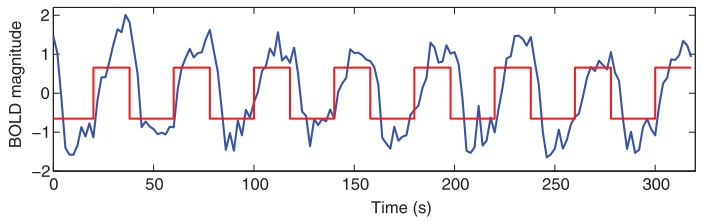
\includegraphics[width=.69\textwidth]{figures/aBackground/stimuli_vs_response}  
	\caption{Figure showing an induced series of stimuli (red) and the hemodynamic response to the neural activity measured using BOLD (blue). It is shown that the measurable hemodynamic response is delayed compared to the stimuli. \cite{Poldrack2011}}
	\label{fig:back:stim} 
\end{figure}


As established in the above section the BOLD signal is effected by the neural activity producing changes in the local blood flow, blood volume and blood oxygenation. The crucial part to why MRI can detect this natural contrast, is that fully oxygenated blood, is diamagnetic and fully deoxygenated blood has four unpaired electrons thereby making it highly paramagnetic. Thereby more oxygenated blood in the area the larger the contrast, compared to other brain regions, is seen as illustrated in \figref{fig:back:bold}. \cite{Glover2011,Khanna2015,Poldrack2011}

\begin{figure}[H]                 
	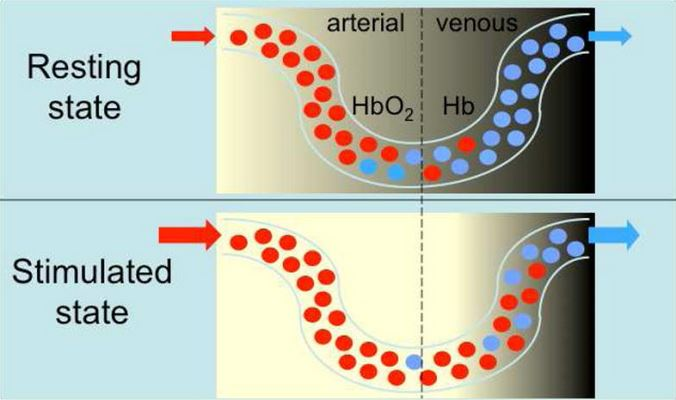
\includegraphics[width=.52\textwidth]{figures/aBackground/bold_response}  
	\caption{Illustration of how the difference in oxygen concentration in the hemoglobin change the magnetic properties, resulting in a higher measurable contrast \cite{Glover2011}.}
	\label{fig:back:bold} 
\end{figure}

This change in local magnetic properties increases the magnetic susceptibility leading to a greater MRI signal when acquiring an $T_2^*$- weighted sequence.  

\section{Standard MRI pre-processing}
There are multiple ways to preprocess fMRI images, some depending on the apparent application. However, there is a standard set of methods that is mostly usually used across all applications. The following section seek to elucidate some of the most commonly used correction methods including the ones considered for the standard preprocessing method used in this project. 

\subsection{Techniques for quality control}
Conducting a continues appropriate quality control is highly recommended to do across all applications, as the example on \figref page 35 shows. Various scanner artifacts can occur while acquiring an MRI series. Spike artifacts are seen as a regular pattern of change in brightness across the entire image. This problem can occur due to instability inside the scanner derivering e.g. from electrical discharges.  
The artifact called ghosting can occur mainly due to two reasons. One being an offset in phase between different lines in K-space and the other due to periodic motion as in heartbeat and respiration. Ghosting can be seen as light copies of the object appearing to either side of the object. Both types of artifacts can corrupt the information contained in the images. However, artifacts of this kind rarely present themselves in newer scanners, nevertheless it is still recommended to control the quality of the scan. \cite{Handbook}

\subsection{Distortion correction}

Some fMRI acquisition methods, including the most widely used method of gradient-echo echo planar imaging, suffers from artifacts at regions air and tissue meet. This could be the areas of ear canal and sinuses. Inhomogeneity in the magnetic field in these areas can cause two types of artifacts, dropout and geometric distortion. A dropout will result in a reduced signal intensity in region close to the air to tissue passage. When a dropout during an acquisition occurs the lost signal cannot be restored and the damage is permanent. Therefore it is wise to consider the appropriate acquisition method taking the area of interest into addition. Air to tissue passages can also be subject to spatial distortion due to inhomogeneity created in the magnetic field. This will lead to structures not being located correctly in the captured image. This distortion makes is difficult to align two different scan, as done when aligning fMRI images with structural images. 
The spatial distortion can partially be corrected by employing field maps. In order to do a field map, the pulse sequences from the scan are needed. The process involved acquiring images at two different echo times. This result in images with two different phases which can be used to compute the field inhomogeneity. Thereby it becomes possible to calculate the relative distance each voxel has shifted. This makes up a map for the distance shift for each voxel, and by inverting the map the original image can be restored.  

\subsection{Slice timing correction}

Acquiring fMRI scans is nearly always done in two-dimensions, where the slices are taken one by one. This can either be in an ascending, descending or interleaved order. Interleaved order \fxnote{think it is done to avoid crosstalk} is sequentially skipping every either odd or even slice and then afterwards do to skipped slices. Regardless of which order the slices are acquired, a difference in effect in each slice to the same hemodynamic response will be present due to the time difference in the slices. The difference in time between slices can range up to a couple of seconds depending on the acquisition protocol. 
The difference in slice timing constitutes a problem when analyzing the data. The data is formed into statistical model, but since this model assumes that all slices are acquired at the same time point, the actual signal and the model creates a mismatch. To counter this problem slice timing correction was introduced. The common approach in this method is to choose a reference slice, usually the slice acquired at T/2, and use this slice to interpolate the others. Linear interpolation can be used for simplicity, but most often sinc interpolation is used as it imposes less smoothing to the signal. 

\subsection{Motion correction}

Having to deal with motion artifacts when doing MRI is inevitable, since even the best subjects will not be able to hold still. Even subtle movements as swallowing will be visible in the raw acquired image. 

Multiple internal and external factors can cause a subject to move. Internal factors are physiologic motion. The heartbeat causes a pulsating movement which makes the brain move. Additionally motion created during respiration can cause small changes in the magnetic field around the head. External factors like imposed stimulus might cause the subject to make sudden movements. Often when doing fMRI the brain activation is measured while the subject is subjected to some kind stimulus. The stimulus would make the patient move, while the brain center would be active, therefore it is easy to mistake brain activation with stimulus correlated movement when analysing the data, resulting in a weaker/false statistical analysis. 

Motion during image acquisition can result in two primary effects, being Bulk motion and Spin history. Bulk motion refers to the movement of the head as a whole and requires standard correction methods, e.g. the images throughout the series to be realigned to a reference image. The effect of Bulk motion can be visual in the entire image of the brain, but the effect will be most predominant at the edges of the brain. Here the artifact will be noticeable as either a drop or increase in intensity as a voxel would switch from containing brain tissue to suddenly not, during head motion.  
Spin history is associated head movement interfering with MRI signal. The interference occur during acquisition when a voxel of excited protons are moved in to a neighbouring slice. The scanner will thereby receive a different signal than expected which is not correctly represent the actual tissue properties. This results in an image where the intensities change in a striped pattern, visible when acquiring slices in interleaved order. The standard motion correction methods cannot cope with this type of artifact, but Independent Component Analysis (ICA) might be to correct for this artifact. 

Motion correction techniques on monday 

\subsection{Spatial smoothing}




	
\urlstyle{same}
\printbibliography
\clearpage



\cleardoublepage
% BILAG
%\begin{appendices}
%	\chapter{Appendices}
%
%\end{appendices}


\end{document}
